\documentclass[12pt]{article}
%%%%%%%%%%%%%%%%
% Packages
%%%%%%%%%%%%%%%%

\usepackage[top=2cm,bottom=2cm,left=2cm,right= 2cm]{geometry}
\usepackage[parfill]{parskip}
\usepackage{graphicx, fontspec, xcolor,multicol, enumitem, setspace, amsmath, changepage}
\DeclareGraphicsRule{.tif}{png}{.png}{`convert #1 `dirname #1`/`basename #1 .tif`.png}

%%%%%%%%%%%%%%%%
% User defined colors
%%%%%%%%%%%%%%%%

% Pantone 2015 Fall colors
% http://iwork3.us/2015/02/18/pantone-2015-fall-fashion-report/
% update each semester or year

\xdefinecolor{custom_blue}{rgb}{0, 0.32, 0.48} % FROM SPRING 2016 COLOR PREVIEW
\xdefinecolor{custom_darkBlue}{rgb}{0.20, 0.20, 0.39} % Reflecting Pond  
\xdefinecolor{custom_orange}{rgb}{0.96, 0.57, 0.42} % Cadmium Orange
\xdefinecolor{custom_green}{rgb}{0, 0.47, 0.52} % Biscay Bay
\xdefinecolor{custom_red}{rgb}{0.58, 0.32, 0.32} % Marsala

\xdefinecolor{custom_lightGray}{rgb}{0.78, 0.80, 0.80} % Glacier Gray
\xdefinecolor{custom_darkGray}{rgb}{0.35, 0.39, 0.43} % Stormy Weather

%%%%%%%%%%%%%%%%
% Color text commands
%%%%%%%%%%%%%%%%

%orange
\newcommand{\orange}[1]{\textit{\textcolor{custom_orange}{#1}}}

% yellow
\newcommand{\yellow}[1]{\textit{\textcolor{yellow}{#1}}}

% blue
\newcommand{\blue}[1]{\textit{\textcolor{blue}{#1}}}

% green
\newcommand{\green}[1]{\textit{\textcolor{custom_green}{#1}}}

% red
\newcommand{\red}[1]{\textit{\textcolor{custom_red}{#1}}}

%%%%%%%%%%%%%%%%
% Coloring titles, links, etc.
%%%%%%%%%%%%%%%%

\usepackage{titlesec}
\titleformat{\section}
{\color{custom_blue}\normalfont\Large\bfseries}
{\color{custom_blue}\thesection}{1em}{}
\titleformat{\subsection}
{\color{custom_blue}\normalfont}
{\color{custom_blue}\thesubsection}{1em}{}

\newcommand{\ttl}[1]{ \textsc{{\LARGE \textbf{{\color{custom_blue} #1} } }}}

\newcommand{\tl}[1]{ \textsc{{\large \textbf{{\color{custom_blue} #1} } }}}

\usepackage[colorlinks=false,pdfborder={0 0 0},urlcolor= custom_orange,colorlinks=true,linkcolor= custom_orange, citecolor= custom_orange,backref=true]{hyperref}

%%%%%%%%%%%%%%%%
% Instructions box
%%%%%%%%%%%%%%%%

\newcommand{\inst}[1]{
\colorbox{custom_blue!20!white!50}{\parbox{\textwidth}{
	\vskip10pt
	\leftskip10pt \rightskip10pt
	#1
	\vskip10pt
}}
\vskip10pt
}

%%%%%%%%%%%
% App Ex number    %
%%%%%%%%%%%

% DON'T FORGET TO UPDATE

\newcommand{\appno}[1]
{1.4}

%%%%%%%%%%%%%%
% Turn on/off solutions       %
%%%%%%%%%%%%%%

% Off
\newcommand{\soln}[2]{$\:$\\ \vspace{#1}}{}

%%% On
%\newcommand{\soln}[2]{\textit{\textcolor{custom_red}{#2}}}{}

%%%%%%%%%%%%%%%%
% Document
%%%%%%%%%%%%%%%%

\begin{document}
\fontspec[Ligatures=TeX]{Helvetica Neue Light}

Dr. \c{C}etinkaya-Rundel \hfill Sta 101: Data Analysis and Statistical Inference \\
Duke University - Department of Statistical Science \hfill \\

\ttl{Application exercise \appno{}: \\
Randomization testing}

\inst{$\:$ \\
Team name: \rule{10cm}{0.5pt} \\
$\:$ \\
Lab section: $\qquad$ 8:30 $\qquad$ 10:05 $\qquad$ 11:45 $\qquad$ 1:25 $\qquad$ 3:05 \\
$\:$ \\
Write your responses in the spaces provided below. WRITE LEGIBLY and SHOW ALL WORK! 
Only one submission per team is required. One team will be randomly selected and their 
responses will be discussed and graded. Concise and coherent are best!}

Student-to-faculty ratio data collected from random samples of public and private four-year colleges:

\begin{minipage}[c]{0.4\textwidth}
\begin{center}
\begin{tabular}{lrrr}
  \hline
type & mean & SD & n \\ 
  \hline
private & 13.84 & 7.28 &  85 \\ 
  public & 17.60 & 4.57 &  57 \\ 
   \hline
\end{tabular}
\end{center}
\end{minipage}
\begin{minipage}[c]{0.6\textwidth}
\begin{center}
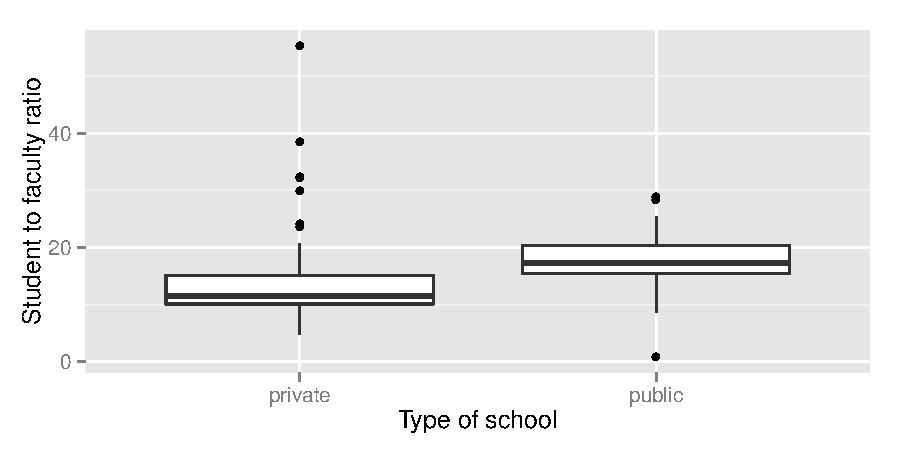
\includegraphics[width=0.8\textwidth]{ratio/ratio_box.pdf}
\end{center}
\end{minipage}


\begin{enumerate}

\item We would like to test if there is a \emph{difference} between the average student-to-faculty ratio between public and private four-year colleges using a randomization test. What are the hypotheses?

\soln{0.5cm}{$H_0: \mu_{public} = \mu_{private}$; $H_0: \mu_{public} \ne \mu_{private}$}

\item Fill in the blanks below for the appropriate set up for this test:

\begin{doublespace}
We write the student-to-faculty ratio of each public and private college in this sample on a total of \rule{2cm}{0.5pt} index cards. Then, we shuffle these cards and split them into two groups: one group of size \rule{2cm}{0.5pt} representing public colleges, and another group of size \rule{2cm}{0.5pt} representing private colleges. We calculate the difference between the average student-to-faculty ratios in the public and private colleges ($\bar{x}_{public} - \bar{x}_{private}$) and record this value. We repeat this many times to build a randomization distribution, which should be centered at \rule{2cm}{0.5pt} . Lastly, we calculate the p-value as the proportion of simulations where the simulated differences in means are \rule{5cm}{0.5pt}.
\end{doublespace}

\soln{0cm}{142, 57, 85, 0, -4 or less or 4 or more}

\item The dot plot below is created using 100 simulations. What is the p-value?

\begin{center}
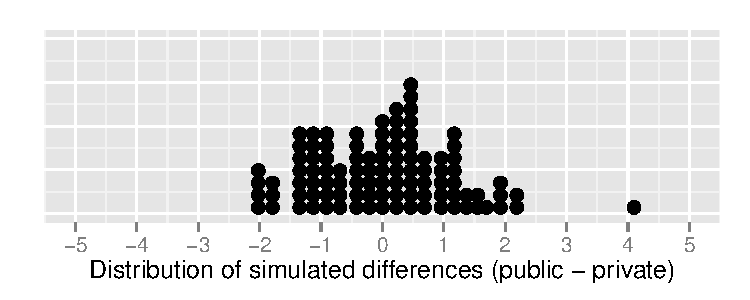
\includegraphics[width=0.8\textwidth]{ratio/rand_dist_dot.pdf}
\end{center}

\soln{0.2cm}{Since only one observation is below -4 or above 4, p-value = 1 / 100 = 0.01.}

\item Based on the p-value, do these data provide convincing evidence to suggest that the student-to-faculty ratio in public four-year colleges is different than that of private four-year colleges.

\soln{1cm}{Yes, p-value is small (less than 0.05), hence we reject the null hypothesis. The data provide convincing evidence that the average student-to-faculty ratio is different for private and public colleges.}

\end{enumerate}

\end{document}